\documentclass[12pt]{article}
\usepackage[left=2cm,right=2cm,top=1cm,bottom=1cm,bindingoffset=0cm]{geometry}
\usepackage[utf8x]{inputenc}
\usepackage[english,russian]{babel}
\usepackage{cmap}
\usepackage{amssymb}
\usepackage{amsmath}
\usepackage{pifont}
\usepackage{tikz}
\usepackage{verbatim}
\usepackage{enumitem}
\usepackage{graphicx}
\usepackage{grffile}

\graphicspath{ {./fig/} }

\pagenumbering{gobble}

\begin{document}

\begin{center}
{\LARGE Формальные языки}

{\Large Контрольная работа 1}

{\large 16.10.2020}
\end{center}

\bigskip


\begin{enumerate}
\setlength\itemsep{1em}

  \item Привести три самых коротких различных строки, принадлежащих языку, описанному регулярным выражением; принадлежат ли строки $abbab$ и $bababa$ данному языку?
  \begin{enumerate}[label=\arabic*)]
    \setlength\itemsep{0.8em}
    \item $a ((a \mid b)^* b)^* $
    \begin{itemize}
      \item $a, ab, abb/aab$, $abbab$ --- yes, $bababa$ --- no.
    \end{itemize}
    \item $(a (a \mid b)^*)^* b $
    \begin{itemize}
      \item $b, ab, aab/abb$, $abbab$ --- yes, $bababa$ --- no.
    \end{itemize}
    \item $(a \mid b) (a (a \mid b))^* (a \mid b) $
    \begin{itemize}
      \item $aa, ab, ba, bb, aaa, aab, baa, bab$, $abbab$ --- no, $bababa$ --- yes.
    \end{itemize}
    \item $(a \mid b) ((a \mid b) b)^* (a \mid b) $
    \begin{itemize}
      \item $aa, ab, ba, bb, aba, abb, bba, bbb$, $abbab$ --- no, $bababa$ --- yes.
    \end{itemize}
    \item $(ba \mid b)^* \mid (bb \mid a)^*$
    \begin{itemize}
      \item $\varepsilon, b, a$, $abbab$ --- no, $bababa$ --- yes.
    \end{itemize}
    \item $(ab \mid b)^* \mid (bb \mid a)^*$
    \begin{itemize}
      \item $\varepsilon, a, b$, $abbab$ --- yes, $bababa$ --- no.
    \end{itemize}
    \item $(ba \mid a)^* \mid (bb \mid a)^*$
    \begin{itemize}
      \item $\varepsilon, a, ba, bb, aa$, $abbab$ --- no, $bababa$ --- yes.
    \end{itemize}
    \item $(ba \mid a)^* \mid (bb \mid b)^*$
    \begin{itemize}
      \item $\varepsilon, a, b$, $abbab$ --- no, $bababa$ --- yes.
    \end{itemize}
    \item $(a \mid b)^* b (a \mid \varepsilon) b (a \mid b)^*$
    \begin{itemize}
      \item $bb, abb, bab, bba, bbb$, $abbab$ --- yes, $bababa$ --- yes.
    \end{itemize}
    \item $(a \mid b)^* a (a \mid \varepsilon) b (a \mid b)^*$
    \begin{itemize}
      \item $ab, aaa, aab, aba, abb, bab,$, $abbab$ --- yes, $bababa$ --- yes.
    \end{itemize}
    \item $(a \mid b)^* b (a \mid \varepsilon) a (a \mid b)^*$
    \begin{itemize}
      \item $ba, aba, baa, bab, bba$, $abbab$ --- yes, $bababa$ --- yes.
    \end{itemize}
    \item $(a \mid b)^* a (a \mid \varepsilon) a (a \mid b)^*$
    \begin{itemize}
      \item $aa, aaa, aab, baa$, $abbab$ --- no, $bababa$ --- no.
    \end{itemize}
    \item $(a \mid b)^* b (b \mid \varepsilon) b (a \mid b)^*$
    \begin{itemize}
      \item $bb, abb, bba, bbb$, $abbab$ --- yes, $bababa$ --- no.
    \end{itemize}
    \item $(a \mid b)^* a (b \mid \varepsilon) b (a \mid b)^*$
    \begin{itemize}
      \item $ab, aab, aba, abb, bab$, $abbab$ --- yes, $bababa$ --- yes.
    \end{itemize}
    \item $(a \mid b)^* b (b \mid \varepsilon) a (a \mid b)^*$
    \begin{itemize}
      \item $ba, aba, baa, bab, bba$, $abbab$ --- yes, $bababa$ --- yes.
    \end{itemize}
    \item $(a \mid b)^* a (b \mid \varepsilon) a (a \mid b)^*$
    \begin{itemize}
      \item $aa, aaa, aab, aba, baa$, $abbab$ --- no, $bababa$ --- yes.
    \end{itemize}
  \end{enumerate}

  \item Построить минимальный детерминированный конечный автомат, распознающий язык:
  \begin{enumerate}[label=\arabic*)]
    \setlength\itemsep{0.8em}
    \item $\{ \omega \cdot a \cdot b \mid \omega \in \{0, 1\}^*, a \in \{0, 1\}, b \in \{0, 1\}, a \ or \ b = 1 \}$
    \begin{itemize}
      \item $ (0 \mid 1)^* 0 1 \mid (0 \mid 1)^* 1 0 \mid (0 \mid 1)^* 1 1$

      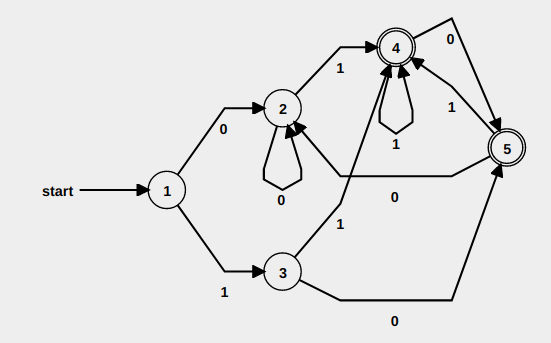
\includegraphics[width=0.5\textwidth]{2.1.png}
    \end{itemize}
    \item $\{ \omega \cdot a \cdot b \mid \omega \in \{0, 1\}^*, a \in \{0, 1\}, b \in \{0, 1\}, a \ and \ b = 0 \}$
    \begin{itemize}
      \item $ (0 \mid 1)^* 0 1 \mid (0 \mid 1)^* 1 0 \mid (0 \mid 1)^* 0 0$

      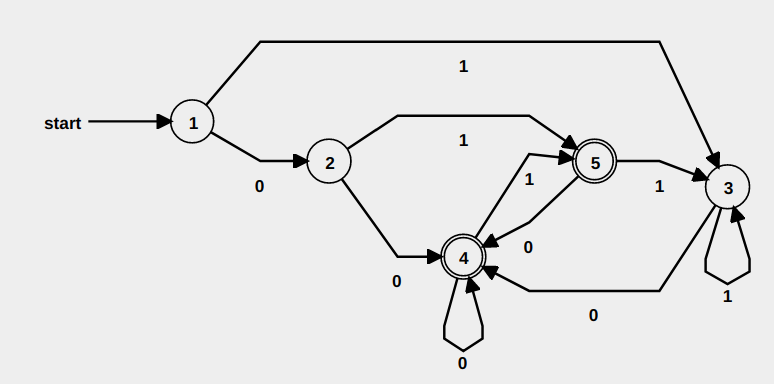
\includegraphics[width=0.5\textwidth]{2.2.png}
    \end{itemize}

    \item $\{ a \cdot \omega \cdot b \mid \omega \in \{0, 1\}^*, a \in \{0, 1\}, b \in \{0, 1\}, a \ or \ b = 1 \}$
    \begin{itemize}
      \item $ 0 (0 \mid 1)^* 1 \mid 1 (0 \mid 1)^* 0 \mid 1 (0 \mid 1)^* 1$

      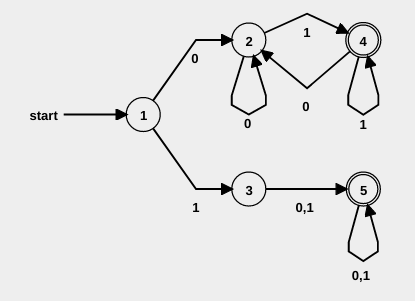
\includegraphics[width=0.5\textwidth]{2.3.png}
    \end{itemize}

    \item $\{ a \cdot \omega \cdot b \mid \omega \in \{0, 1\}^*, a \in \{0, 1\}, b \in \{0, 1\}, a \ and \ b = 0 \}$
    \begin{itemize}
      \item $0 (0 \mid 1)^* 1 \mid 1 (0 \mid 1)^* 0 \mid 0 (0 \mid 1)^* 0 $

      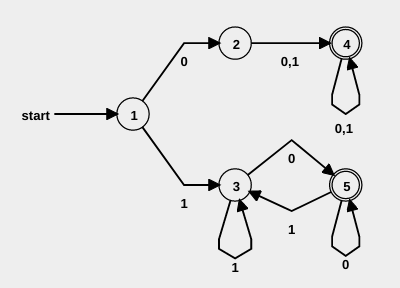
\includegraphics[width=0.5\textwidth]{2.4.png}
    \end{itemize}
    \item $\{ a \cdot b \cdot \omega \mid \omega \in \{0, 1\}^*, a \in \{0, 1\}, b \in \{0, 1\}, a \ or \ b = 1 \}$
    \begin{itemize}
      \item $0 1 (0 \mid 1)^* \mid 1 0 (0 \mid 1)^* \mid 1 1 (0 \mid 1)^* $

      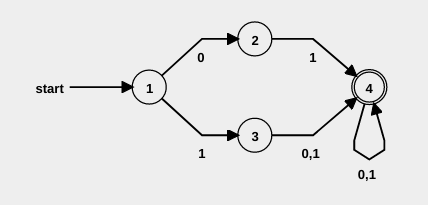
\includegraphics[width=0.5\textwidth]{2.5.png}
    \end{itemize}
    \item $\{ a \cdot b \cdot \omega \mid \omega \in \{0, 1\}^*, a \in \{0, 1\}, b \in \{0, 1\}, a \ and \ b = 0 \}$
    \begin{itemize}
      \item $  0 1 (0 \mid 1)^* \mid 1 0  (0 \mid 1)^* \mid 0 0 (0 \mid 1)^* $

      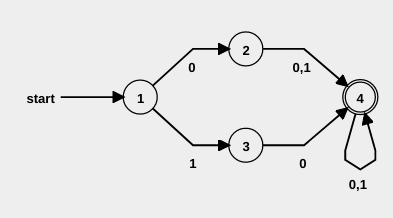
\includegraphics[width=0.5\textwidth]{2.6.png}
    \end{itemize}


    \item $\{ \omega \cdot a \cdot b \mid \omega \in \{0, 1\}^*, a \in \{0, 1\}, b \in \{0, 1\}, a = b \}$
    \begin{itemize}
      \item $ (0 \mid 1)^* 00 \mid (0 \mid 1)^* 11 $

      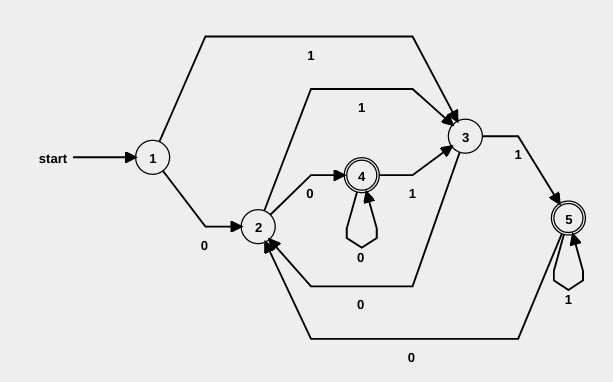
\includegraphics[width=0.5\textwidth]{2.7.png}
    \end{itemize}
    \item $\{ \omega \cdot a \cdot b \mid \omega \in \{0, 1\}^*, a \in \{0, 1\}, b \in \{0, 1\}, a \neq b \}$
    \begin{itemize}
      \item $ (0 \mid 1)^* 01 \mid (0 \mid 1)^* 10 $

      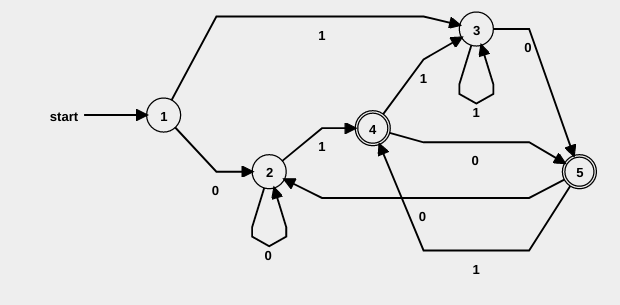
\includegraphics[width=0.5\textwidth]{2.8.png}
    \end{itemize}
    \item $\{ a \cdot \omega \cdot b \mid \omega \in \{0, 1\}^*, a \in \{0, 1\}, b \in \{0, 1\}, a = b \}$
    \begin{itemize}
      \item $ 0(0 \mid 1)^* 0\mid 1(0 \mid 1)^*1 $

      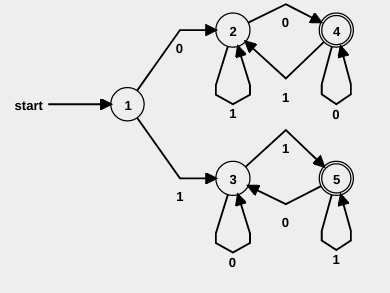
\includegraphics[width=0.5\textwidth]{2.9.png}
    \end{itemize}
    \item $\{ a \cdot \omega \cdot b \mid \omega \in \{0, 1\}^*, a \in \{0, 1\}, b \in \{0, 1\}, a \neq b \}$
    \begin{itemize}
      \item $0 (0 \mid 1)^* 1\mid 1 (0 \mid 1)^* 0$

      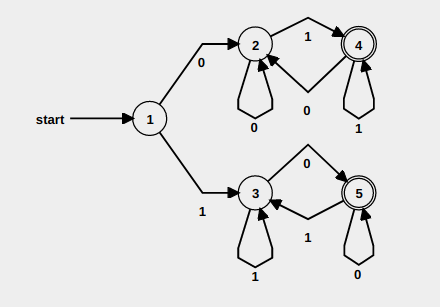
\includegraphics[width=0.5\textwidth]{2.10.png}
    \end{itemize}
    \item $\{ a \cdot b \cdot \omega \mid \omega \in \{0, 1\}^*, a \in \{0, 1\}, b \in \{0, 1\}, a = b \}$
    \begin{itemize}
      \item $ 0 0 (0 \mid 1)^* \mid 1 1 (0 \mid 1)^* $

      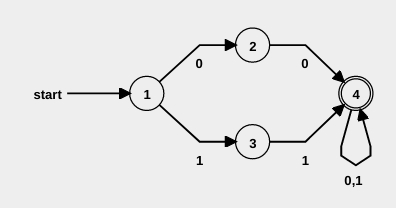
\includegraphics[width=0.5\textwidth]{2.11.png}
    \end{itemize}
    \item $\{ a \cdot b \cdot \omega \mid \omega \in \{0, 1\}^*, a \in \{0, 1\}, b \in \{0, 1\}, a \neq b \}$
    \begin{itemize}
      \item $ 0 1 (0 \mid 1)^* \mid 1 0 (0 \mid 1)^* $

      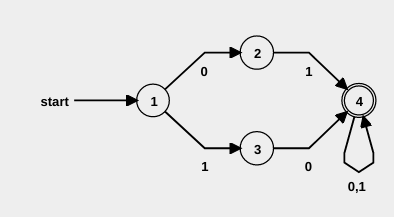
\includegraphics[width=0.5\textwidth]{2.12.png}
    \end{itemize}

  \end{enumerate}

  \item Построить регулярную грамматику, задающую язык:
  \begin{enumerate}[label=\arabic*)]
    \setlength\itemsep{0.8em}

    \item $\{ \alpha \cdot 100 \cdot \beta \mid \alpha, \beta \in \{0, 1\}^*\} \cap \{\gamma \cdot 000 \cdot \delta \mid \gamma, \delta \in \{0, 1\}^* \}$
    \begin{itemize}
      \item $\xi 000 \xi 100 \xi \mid \xi 100 \xi 000 \xi \mid \xi 1000 \xi $
    \end{itemize}
    \item $\{ \alpha \cdot 100 \cdot \beta \mid \alpha, \beta \in \{0, 1\}^*\} \cup \{\gamma \cdot 000 \cdot \delta \mid \gamma, \delta \in \{0, 1\}^* \}$
    \begin{itemize}
      \item $\xi 100 \xi \mid \xi 000 \xi $
    \end{itemize}
    \item $\{ \alpha \cdot 001 \cdot \beta \mid \alpha, \beta \in \{0, 1\}^*\} \cap \{\gamma \cdot 000 \cdot \delta \mid \gamma, \delta \in \{0, 1\}^* \}$
    \begin{itemize}
      \item $\xi 001 \xi 000 \xi \mid \xi 000 \xi 001 \xi \mid \xi 0001 \xi $
    \end{itemize}
    \item $\{ \alpha \cdot 001 \cdot \beta \mid \alpha, \beta \in \{0, 1\}^*\} \cup \{\gamma \cdot 000 \cdot \delta \mid \gamma, \delta \in \{0, 1\}^* \}$
    \begin{itemize}
      \item $\xi 001 \xi \mid \xi 000 \xi $
    \end{itemize}
    \item $\{ \alpha \cdot 010 \cdot \beta \mid \alpha, \beta \in \{0, 1\}^*\} \cap \{\gamma \cdot 000 \cdot \delta \mid \gamma, \delta \in \{0, 1\}^* \}$
    \begin{itemize}
      \item $\xi 010 \xi 000 \xi \mid \xi 000 \xi 010 \xi \mid \xi 00010 \xi \mid \xi 01000 $
    \end{itemize}
    \item $\{ \alpha \cdot 010 \cdot \beta \mid \alpha, \beta \in \{0, 1\}^*\} \cup \{\gamma \cdot 000 \cdot \delta \mid \gamma, \delta \in \{0, 1\}^* \}$
    \begin{itemize}
      \item $\xi 010 \xi \mid \xi 000 \xi $
    \end{itemize}
    \item $\{ \alpha \cdot 001 \cdot \beta \mid \alpha, \beta \in \{0, 1\}^*\} \cap \{\gamma \cdot 100 \cdot \delta \mid \gamma, \delta \in \{0, 1\}^* \}$
    \begin{itemize}
      \item $\xi 001 \xi 100 \xi \mid \xi 100 \xi 001 \xi \mid \xi 00100 \xi \mid \xi 1001 \xi \mid \xi 10001\xi  $
    \end{itemize}
    \item $\{ \alpha \cdot 001 \cdot \beta \mid \alpha, \beta \in \{0, 1\}^*\} \cup \{\gamma \cdot 100 \cdot \delta \mid \gamma, \delta \in \{0, 1\}^* \}$
    \begin{itemize}
      \item $\xi 001 \xi \mid \xi 100 \xi $
    \end{itemize}
    \item $\{ \alpha \cdot 101 \cdot \beta \mid \alpha, \beta \in \{0, 1\}^*\} \cap \{\gamma \cdot 010 \cdot \delta \mid \gamma, \delta \in \{0, 1\}^* \}$
    \begin{itemize}
      \item $\xi 101 \xi 010 \xi \mid \xi 010 \xi 101 \xi \mid \xi 0101 \xi \mid \xi 1010 \xi $
    \end{itemize}
    \item $\{ \alpha \cdot 101 \cdot \beta \mid \alpha, \beta \in \{0, 1\}^*\} \cup \{\gamma \cdot 010 \cdot \delta \mid \gamma, \delta \in \{0, 1\}^* \}$
    \begin{itemize}
      \item $\xi 101 \xi \mid \xi 010 \xi $
    \end{itemize}

    \item $\{ \alpha \cdot 011 \cdot \beta \mid \alpha, \beta \in \{0, 1\}^*\} \cap \{\gamma \cdot 111 \cdot \delta \mid \gamma, \delta \in \{0, 1\}^* \}$
    \begin{itemize}
      \item $\xi 011 \xi 111 \xi \mid \xi 111 \xi 011 \xi \mid \xi 0111 \xi $
    \end{itemize}
    \item $\{ \alpha \cdot 011 \cdot \beta \mid \alpha, \beta \in \{0, 1\}^*\} \cup \{\gamma \cdot 111 \cdot \delta \mid \gamma, \delta \in \{0, 1\}^* \}$
    \begin{itemize}
      \item $\xi 011 \xi \mid \xi 111 \xi $
    \end{itemize}
    \item $\{ \alpha \cdot 110 \cdot \beta \mid \alpha, \beta \in \{0, 1\}^*\} \cap \{\gamma \cdot 111 \cdot \delta \mid \gamma, \delta \in \{0, 1\}^* \}$
    \begin{itemize}
      \item $\xi 110 \xi 111 \xi \mid \xi 111 \xi 110 \xi \mid \xi 1110 \xi $
    \end{itemize}
    \item $\{ \alpha \cdot 110 \cdot \beta \mid \alpha, \beta \in \{0, 1\}^*\} \cup \{\gamma \cdot 111 \cdot \delta \mid \gamma, \delta \in \{0, 1\}^* \}$
    \begin{itemize}
      \item $\xi 110 \xi \mid \xi 111 \xi $
    \end{itemize}
    \item $\{ \alpha \cdot 101 \cdot \beta \mid \alpha, \beta \in \{0, 1\}^*\} \cap \{\gamma \cdot 111 \cdot \delta \mid \gamma, \delta \in \{0, 1\}^* \}$
    \begin{itemize}
      \item $\xi 101 \xi 111 \xi \mid \xi 111 \xi 101 \xi \mid \xi 11101 \xi \mid \xi 10111 \xi $
    \end{itemize}
    \item $\{ \alpha \cdot 101 \cdot \beta \mid \alpha, \beta \in \{0, 1\}^*\} \cup \{\gamma \cdot 111 \cdot \delta \mid \gamma, \delta \in \{0, 1\}^* \}$
    \begin{itemize}
      \item $\xi 101 \xi \mid \xi 111 \xi $
    \end{itemize}
    \item $\{ \alpha \cdot 110 \cdot \beta \mid \alpha, \beta \in \{0, 1\}^*\} \cap \{\gamma \cdot 011 \cdot \delta \mid \gamma, \delta \in \{0, 1\}^* \}$
    \begin{itemize}
      \item $\xi 110 \xi 011 \xi \mid \xi 011 \xi 110 \xi \mid \xi 01110 \xi \mid \xi 0110 \xi \mid \xi 11011 \xi$
    \end{itemize}
    \item $\{ \alpha \cdot 110 \cdot \beta \mid \alpha, \beta \in \{0, 1\}^*\} \cup \{\gamma \cdot 011 \cdot \delta \mid \gamma, \delta \in \{0, 1\}^* \}$
    \begin{itemize}
      \item $\xi 110 \xi \mid \xi 011 \xi $
    \end{itemize}
    \item $\{ \alpha \cdot 010 \cdot \beta \mid \alpha, \beta \in \{0, 1\}^*\} \cap \{\gamma \cdot 101 \cdot \delta \mid \gamma, \delta \in \{0, 1\}^* \}$
    \begin{itemize}
      \item $\xi 010 \xi 101 \xi \mid \xi 101 \xi 010 \xi \mid \xi 1010 \xi \mid \xi 0101 \xi$
    \end{itemize}
    \item $\{ \alpha \cdot 010 \cdot \beta \mid \alpha, \beta \in \{0, 1\}^*\} \cup \{\gamma \cdot 101 \cdot \delta \mid \gamma, \delta \in \{0, 1\}^* \}$
    \begin{itemize}
      \item $\xi 010 \xi \mid \xi 101 \xi $
    \end{itemize}
  \end{enumerate}

  \item Проверить регулярность языка (если регулярный, построить автомат, регулярное выражение или регулярную грамматику, иначе --- доказать нерегулярность)
  \begin{enumerate}[label=\arabic*)]
    \setlength\itemsep{0.8em}

    \item $\{\omega \in \{a, b\}^* \mid |\omega|_a = |\omega|_b\}$
    \item $\{\omega \in \{a, b\}^* \mid |\omega|_a \geq |\omega|_b\}$
    \item $\{\omega \in \{a, b\}^* \mid |\omega|_a \leq |\omega|_b\}$
    \item $\{\omega \in \{a, b\}^* \mid |\omega|_a \neq |\omega|_b\}$
    \item $\{\alpha \cdot a \cdot \beta \mid \alpha, \beta \in \{a, b\}^*, |\alpha|_b \geq |\beta|_a \}$
    \item $\{\alpha \cdot a \cdot \beta \mid \alpha, \beta \in \{a, b\}^*, |\alpha|_b > |\beta|_a \}$
    \item $\{a^m \cdot \omega \mid 1 \leq |\omega|_b \leq m\}$
    \item $\{\omega \cdot a^m  \mid 1 \leq |\omega|_b \leq m\}$
  \end{enumerate}

  \item По регулярному выражению построить недетерминированный конечный автомат без эпсилон-переходов
  \begin{enumerate}[label=\arabic*)]
    \setlength\itemsep{0.8em}

    \item $a ((a \mid b)^* b)^* $

    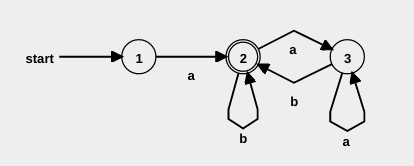
\includegraphics[width=0.5\textwidth]{5.1.png}
    \item $(a (a \mid b)^*)^* b $

    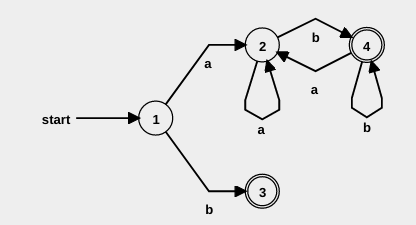
\includegraphics[width=0.5\textwidth]{5.2.png}
    \item $(a \mid b) (a (a \mid b))^* (a \mid b) $

    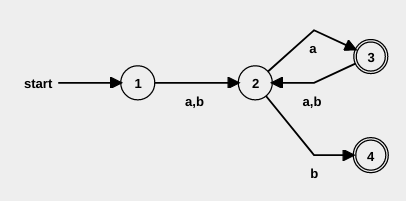
\includegraphics[width=0.5\textwidth]{5.3.png}
    \item $(a \mid b) ((a \mid b) b)^* (a \mid b) $

    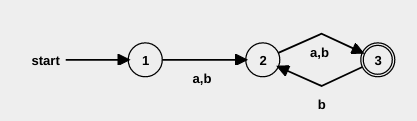
\includegraphics[width=0.5\textwidth]{5.4.png}
    \item $(ba \mid b)^* \mid (bb \mid a)^*$

    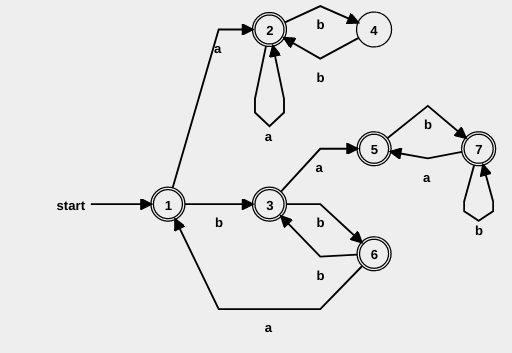
\includegraphics[width=0.5\textwidth]{5.5.png}
    \item $(ab \mid b)^* \mid (bb \mid a)^*$

    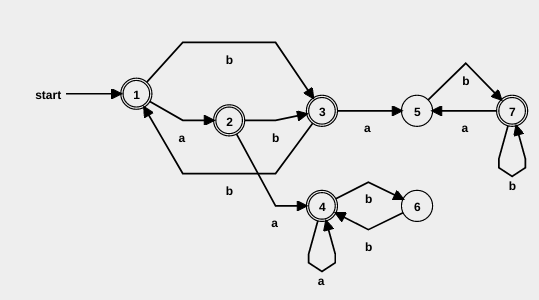
\includegraphics[width=0.5\textwidth]{5.6.png}
    \item $(ba \mid a)^* \mid (bb \mid a)^*$

    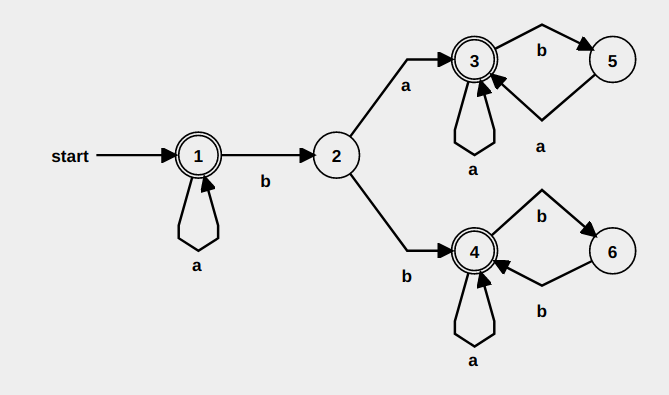
\includegraphics[width=0.5\textwidth]{5.7.png}
    \item $(ba \mid a)^* \mid (bb \mid b)^*$

    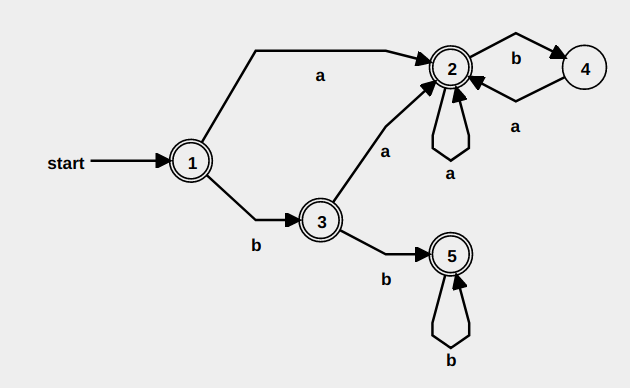
\includegraphics[width=0.5\textwidth]{5.8.png}
    \item $(a \mid b)^* b (a \mid \varepsilon) b (a \mid b)^*$

    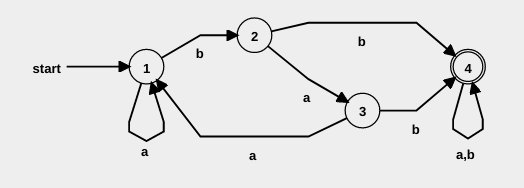
\includegraphics[width=0.5\textwidth]{5.9.png}
    \item $(a \mid b)^* a (a \mid \varepsilon) b (a \mid b)^*$

    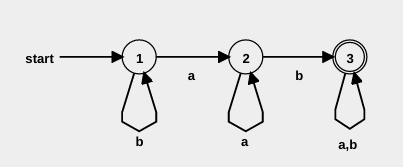
\includegraphics[width=0.5\textwidth]{5.10.png}
    \item $(a \mid b)^* b (a \mid \varepsilon) a (a \mid b)^*$

    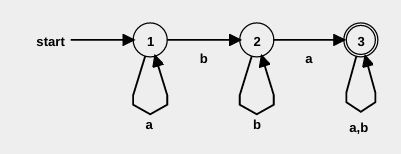
\includegraphics[width=0.5\textwidth]{5.11.png}
    \item $(a \mid b)^* a (a \mid \varepsilon) a (a \mid b)^*$

    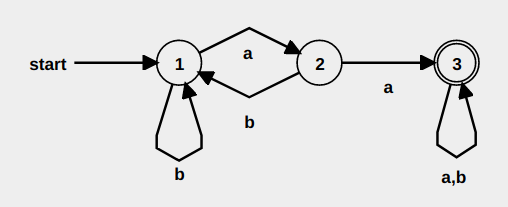
\includegraphics[width=0.5\textwidth]{5.12.png}
    \item $(a \mid b)^* b (b \mid \varepsilon) b (a \mid b)^*$

    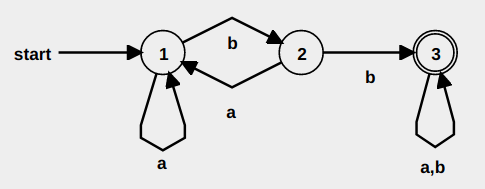
\includegraphics[width=0.5\textwidth]{5.13.png}
    \item $(a \mid b)^* a (b \mid \varepsilon) b (a \mid b)^*$

    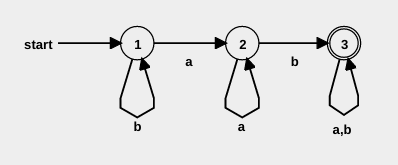
\includegraphics[width=0.5\textwidth]{5.14.png}
    \item $(a \mid b)^* b (b \mid \varepsilon) a (a \mid b)^*$

    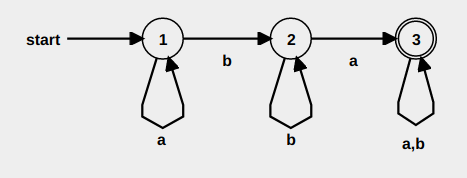
\includegraphics[width=0.5\textwidth]{5.15.png}
    \item $(a \mid b)^* a (b \mid \varepsilon) a (a \mid b)^*$

    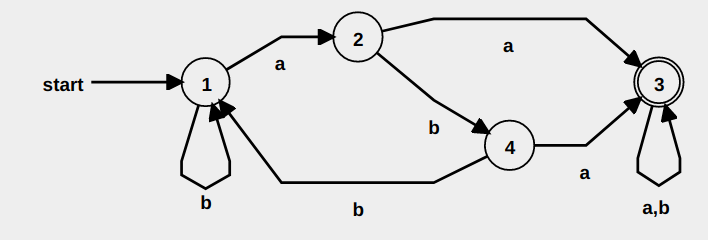
\includegraphics[width=0.5\textwidth]{5.16.png}

  \end{enumerate}
\end{enumerate}

\end{document}
